\documentclass[PhysicsI/physics_notes.tex]{subfiles}
\begin{document}
\section{Aula 07 - 17/03/2023}
\subsection{Motivações}
\begin{itemize}
	\item Começar a estudar o movimento circular;
\end{itemize}

\subsection{Movimento Circular}
Quando temos uma particular fazendo movimento circular em um círculo de raio R num eixo x, y, diremos que ela, sua posição em qualquer instante
será dada por um vetor r(t), sendo sua trajetória limitada a este círculo. Assim, obtemos o sistema $R = |\vec{r}(t)|$, sendo
$\vec{r}(t) = x(t)\hat{i} + y(t)\hat{j}$ e
$$
	\left\{\begin{array}{ll}
		x(t) = R\cos{\theta(t)} \\
		y(t) = R\sin{\theta(t)}.
	\end{array}\right.
$$
\begin{center}
	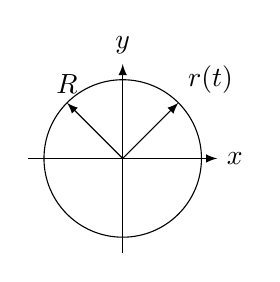
\begin{tikzpicture}[>=latex]
		\draw[->] (-1.2,0) -- (1.2,0) node[right] {$x$};
		\draw[->] (0,-1.2) -- (0,1.2) node[above] {$y$};
		\draw (0,0) circle [radius=1];
		\draw[->] (0, 0) -- ({-cos(45)}, {sin(45)}) node[above] {$R$};
		\draw[->] (0,0) -- ({cos(45)},{sin(45)}) node[above right] {$r(t)$};
	\end{tikzpicture}
\end{center}
Utilizando o sistema e o desenho, obtemos
$$
	\vec{r}(t) = R\cos{\theta(t)}\hat{i} + R\sin{\theta(t)}\hat{j},
$$
donde segue o valor do módulo do vetor $\vec{r}(t)$:
\begin{align*}
	|\vec{r}(t)|^{2} = x^{2}(t) + y^{2}(t) & = (R\cos{\theta(t)})^{2} + (R\sin{\theta(t)})^{2}  \\
	                                       & = R^{2}(\cos{\theta(t)}^{2} + \sin{\theta(t)}^{2}) \\
	                                       & = R^{2} \Rightarrow |\vec{r}(t)| = R.
\end{align*}
Concluímos, assim, que todo o movimento da partícula é dado em termos do ângulo $\theta(t).$ Além disso, o deslocamento
da partícula é feita em arcos de círculo $s(t) = R\theta(t)$. Chamamos esta posição de ``posição escalar do corpo sobre o círculo''.
No entanto, no movimento circular, há outra posição, chamada ``posição angular do corpo'', que é dada por $\theta(t) = \frac{s(t)}{R}.$

Utilizando estes dois, podemos encontrar uma equação para $\vec{r}(t)$:
$$
	\vec{r}(t) = R\cos{\theta(t)}\hat{i} + R\sin{\theta(t)}\hat{j} = R\underbrace{[\cos{\theta(t)}\hat{i} + \sin{\theta(t)}\hat{j}]}_{\hat{r}(t)}
	= R\hat{r}(t),
$$
em que $\hat{r}(t)$ é um versor na direção de $\vec{r}(t)$, isto é, um vetor com módulo um. De fato, vamos verificar isto:
$$
	|\hat{r}(t)| = \sqrt[]{\cos^{2}(\theta(t)) + \sin^{2}(\theta(t))} = 1
$$
A seguir, vamos estudar como este versor $\hat{r}(t)$ varia, ou seja, vamos derivar este vetor com respeito ao tempo. Para isso,
introduizremos outra regra de derivação, a ``Regra da Cadeia''. Dada uma função $f(t) = u(v(t))$, ou seja, uma função
definida como uma função composta, sua derivação é feita de denro pra fora: Derivamos v(t) com respeito a t, depois derivamos
u com relação a v e multiplicamos, ou seja,
$$
	\boxed{\frac{df}{dt} = \frac{du}{dv}\frac{dv}{dt}}.
$$
Assim, no caso do versor $\hat{r}(t),$
\begin{align*}
	\frac{d\hat{r}(t)}{dt} & = \frac{d}{dt}[\cos{\theta(t)}\hat{i} + \sin{\theta(t)}\hat{j}]                                                               \\
	                       & = \frac{d}{dt}[\cos{\theta(t)}]\hat{i} + \frac{d}{dt}[\sin{\theta(t)}]\hat{j}                                                 \\
	                       & = \frac{d\cos{\theta(t)}}{d\theta}\frac{d\theta(t)}{dt}\hat{i} + \frac{d\sin{\theta(t)}}{d\theta}\frac{d\theta(t)}{dt}\hat{j} \\
	                       & = -\sin{\theta(t)}\frac{d\theta(t)}{dt}\hat{i} + \cos{\theta(t)}\frac{d\theta(t)}{dt}\hat{j}.
\end{align*}
Como $\theta(t)$ é a posição angular, chamamos a sua derivada com respeito a tempo de velocidade ângular
$$
	\boxed{\omega(t) = \frac{d\theta(t)}{dt}.}
$$
De brinde, conseguimos definir a velocidade escalar da partícula como
\begin{align*}
	\frac{ds(t)}{dt} & = \frac{dR\theta(t)}{dt} = R \frac{d\theta(t)}{dt} = R\omega(t). \\
	                 & \Rightarrow \boxed{v(t) = R\omega(t).}
\end{align*}
Vamos estudar a dimensão dessa quantidade. Temos
$$
	[\omega] = \frac{[\theta]}{[t]} = \frac{1}{T} \quad \text{(Exemplo: rad/s (radianos por segundo.))}
$$
como unidades de velocidade angular e
$$
	[v] = [R][\omega] = LT^{-1} \quad \text{(Exemplo: m/s (metros por segundo))}
$$
como dimensão da velocidade escalar. Com relação ao versor definido, sua derivada é
$$
	\frac{d\hat{r}(t)}{dt} = \omega(t)\underbrace{[-\sin{\theta(t)}\hat{i}+\cos{\theta(t)}\hat{j}]}_{\hat{\theta(t)}},
$$
em que $\hat{\theta(t)}$ é um versor apontando na direção do ângulo. Com isso, definimos a velocidade vetorial por
$$
	\vec{v}(t) = \frac{d \vec{r}(t)}{dt} = R \frac{d\hat{r}(t)}{dt} \Rightarrow \vec{v}(t) = R\omega(t)\hat{\theta(t)}.
$$
Algo interessante de notar é que a velocidade escalar consiste do módulo da velocidade vetorial, i.e., $v(t) = |\vec{v}(t)|.$
Também podemos representar a velocidade por meio das componentes em cada eixo:
$$
	\vec{v}(t) = \underbrace{-R\omega(t)\sin{\theta(t)}}_{v_{x}(t)}\hat{i} + \underbrace{R\omega(t)\cos{\theta(t)}}_{v_{y}(t)}\hat{j}.
$$
\subsection{Acelerações no Movimento Circular.}
Agora que estamos mais familiariizados com a velocidade e posição angular, podemos estudar a aceleração no movimento circular.
Assim como antes, começamos definindo a aceleração angular:
$$
	\alpha(t) = \frac{d\omega(t)}{dt} = \frac{d^{2}\theta(t)}{dt^{2}},
$$
que possui dimensão $[\alpha] = \frac{[\omega]}{[t]} = \frac{T^{-1}}{T} = T^{-2}$, sendo um exemplo a unidade $rad/s^{2}$, i.e.,
radiano por segundo quadrado. Analogamente, definimos a aceleração vetorial por
$$
	\vec{a}(t) = \frac{d \vec{v}(t)}{dt} = \frac{d}{dt}[R\omega(t)\hat{\theta}(t)].
$$
Pela regra do produto,
$$
	\vec{a}(t) = R[\frac{d\omega(t)}{dt}\hat{\theta(t)} + \omega(t) \frac{d\hat{\theta(t)}}{dt}].
$$
Analisando termo a termo, a primeira derivada acontece no módulo da velocidade, i.e., $R \frac{d\omega(t)}{dt}$, ou seja,
representa a variação no módulo da velocdade. Por outro lado, o segundo termo representa a variação da direção
da velocidade. Como já encontramos alguns desses termos antes, segue que
$$
	\vec{a}(t) = R[\alpha(t)\hat{\theta(t)} + v(t)\frac{d\hat{\theta}(t)}{dt}].
$$
Mas o que é este termo $\frac{d\hat{\theta}}{dt}$? Olhando pra ele com cuidado, vemos que
\begin{align*}
	\frac{d\hat{\theta}}{dt} & = \frac{d}{dt}[-\sin{\theta(t)}\hat{i} + \cos{\theta(t)}\hat{j}]                                                                \\
	                         & = -\frac{d}{dt}[\sin{\theta(t)}]\hat{i} + \frac{d}{dt}[\cos{\theta(t)}]\hat{j}                                                  \\
	                         & = -\cos{\theta(t)}\frac{d\theta(t)}{dt}\hat{i} -\sin{\theta(t)}\frac{d\theta(t)}{dt}\hat{j}                                     \\
	                         & \Rightarrow \frac{d\hat{\theta(t)}}{dt} = \omega(t)[-\cos{\theta(t)}\hat{i} - \sin{\theta(t)}\hat{j}] = \omega(t)(-\hat{r}(t)).
\end{align*}
Portanto,
$$
	\vec{a}(t) = R[\alpha(t)\hat{\theta(t)} + \omega^{2}(t)(-\hat{r}(t))] = \underbrace{R\alpha(t)\hat{\theta(t)}}_{\text{aceleração tangencial }\vec{a}_{t}(t)} - \underbrace{R\omega^{2}(t)\hat{r}(t)}_{\text{aceleração centrípeta }\vec{a}_{cp}(t)}
$$
Obtivemos disso tudo duas acelerações novas e que precisam ser mais compreendidas. Vamos começar pela tangencial.

Com relação ao módulo da aceleração tangencial, note que $|\vec{a}_{t}(t)| = R\alpha(t) = \frac{dv(t)}{dt}$. Agora,
quanto à aceleração centrípeta, seu módulo é dado por $|\vec{a}_{cp}(t)| = R\omega^{2}(t) \Rightarrow|\vec{a}_{cp}(t)| = \frac{v^{2}}{R}.$

\subsection{Movimento Circular Uniforme}
Resumindo o que temos até o momento em forma de tabela, segue que

\begin{table}[h!]
	\centering
	\begin{tabular}{|c|c|c|}
		\hline
		                    & \textbf{Variáveis angulares}                                    & \textbf{Variáveis escalares}                                                        \\
		\hline
		\textbf{Posição}    & $\theta(t)$                                                     & $s(t) = R\theta(t)$                                                                 \\
		\hline
		\textbf{Velocidade} & $\omega(t) = \frac{d \theta(t)}{dt}$                            & $v(t) = \frac{d s(t)}{dt} = R\omega(t)$                                             \\
		\hline
		\textbf{Aceleração} & $\alpha(t) = \frac{d\omega(t)}{dt} = \frac{d^2\theta(t)}{dt^2}$ & $|\vec{a}(t)| = \frac{dv(t)}{dt} = R\alpha(t),\quad |\vec{a}_{cp}| = \frac{v^2}{R}$ \\
		\hline
	\end{tabular}
	\caption{Resumo movimento circular.}
	\label{tab:my_label}
\end{table}
No movimento circular uniforme, estudamos arcos iguais em tempos iguais, ou seja,
$$
	\Delta s_{1} = \Delta s_{2},\quad \Delta t_{1} = \Delta t_{2},
$$
tal que $\Delta \theta_{1} = \Delta \theta_{2}$. Além disos, $\omega(t)\equiv \omega$ constante. Assim,
$$
	|\vec{v}(t)| = v(t) = R\omega(t)\equiv v,\text{ constante} \Rightarrow a_{t} = R\alpha(t) = 0.
$$
Com isso, as posições são descritas por
\begin{align*}
	 & \omega(t) = \omega \Rightarrow \theta(t) = \theta_{0} + \omega(t-t_{0}) \\
	 & v(t) = v \Rightarrow s(t) = s_{0} + v(t-t_{0})
\end{align*}
Neste caso, o movimento é periódico, ou seja, ele volta a ter as mesmas propriedades após um período T. Em forma matemática, isso quer dizer que
$$
	\left\{\begin{array}{ll}
		\vec{r}(t + T) = \vec{r}(t) \\
		\vec{v}(t + T) = \vec{v}(t).
	\end{array}\right.
$$
Tendo isso em mente, definimos também a frequência como o número de ocorrências. Ele vale o inverso do período T, i.e., $f = \frac{1}{T}$.

\end{document}
